%!TEX root=document.tex

\section{Introduction}
\label{sec:introduction}
Data visualization is often the first step in data analysis.
Given a new dataset or a new question about an existing dataset, an analyst builds
various visualizations to get a feel for the data, to find anomalies and outliers, 
and to identify trends and patterns that might merit further investigation.
However, when working with high-dimensional datasets, identifying visualizations that
show interesting variations and trends in data is non-trivial:
the analyst must manually specify a large number of visualizations, explore relationships between various
attributes (and combinations thereof), and examine different subsets of data before finally 
arriving at visualizations that are interesting or insightful.
This need to manually specify and examine every visualization hampers rapid analysis 
and exploration.


In this paper, we tackle the problem of automatically 
identifying and recommending 
visualizations for visual analysis.  
One of the core challenges in recommending visualizations is the fact that 
whether a visualization is interesting or not
depends on a host of factors.
In this paper, we adopt a simple criterion for judging the {\em interestingness} of a visualization: 
a visualization is likely to be interesting if it displays 
{\em large deviations from some
reference} (e.g. another dataset, historical data, or the rest of the data.)
While simple, we find in user studies (Section \ref{sec:user_study}) 
that deviation can often guide users towards visualizations they find interesting.
Of course, there are other elements that may make a visualization interesting.
Examples include aesthetics (as explored in prior work~\cite{polaris,Mackinlay:1986:ADG:22949.22950}), 
the particular attributes of the data being presented 
(our interactive tool allows analysts to choose attributes of interest) 
or other kinds of trends in
data (for example, in some cases, a {\it lack} of deviation may be interesting.)  
Therefore, while our focus is on visualizations with large deviation, 
we develop a system, titled \SeeDB, 
and underlying techniques that are largely agnostic to the
particular definition of interestingness.
In Section~\ref{sec:discussion}, we describe how our system can be
extended to support a generalized utility metric, incorporating
other criteria in addition to deviation. 
\resolved{\mpv{Depending on how we write the extensions section:
we also design a generalized utility metric for evaluating visualization 
quality (in Section 8), and describe how our system is capable of handling
this generalized utility metric for recommending visualizations.
Or: In Section \ref{sec:discussion}, we outline some techniques to extend our
utility metric to incorporate other dimensions of quality and the corresponding...
}}

%it is entirely subjective \mpv{depends on a host of factors}.  
% However, our hypothesis, which we demonstrate
% empirically through user studies, is that many interesting visualizations 
% demonstrate large deviations from some reference data set (we define this notion formally below.)
% Of course, there many other elements that may make a visualization interesting.
% Examples include aesthetics (which we explicitly do not focus on), the particular attributes of the data being
% presented (our interactive tool allows users to choose attributes of interest) or other kinds of trends in
% data (for example, in some cases, a {\it lack} of deviation may be interesting.)  Thus,
% in addition to our focus on visualizations with large deviation, we develop a generalized
% utility metric for evaluating visualization quality, and develop several
% techniques for recommending {\it high utility} visualizations.


Given a particular criteria for interestingness, called the {\em utility metric},
the goal of recommending visualizations based on this metric 
raises several challenges:
first, even for a modest dataset with a small number
of attributes, the number of  
visualizations that need to be considered is often in the hundreds or thousands.
For some datasets, simply generating each of these visualizations can take many minutes 
(as we will see in this paper).
Second, evaluating each of these visualizations for utility requires repeated
computations on the same underlying data, wasting time and computational resources.
Third, recommendations need to be made to analysts at interactive speeds,
necessitating approximations that return visualizations with slightly lower accuracy. 
Addressing challenges and trade-offs in our system, \SeeDB, 
is the primary focus of this paper. 

% first, the curse of dimensionality makes the number of possible visualizations very large;
% second, evaluating the utility of each visualization may require re-running computations over the 
% same underlying data; 
% and third, recommendations must be made to users in real-time, and at interactive speeds.


%Our system, \SeeDB, is designed to address all of these challenges.


% The goal of recommending high-utility visualizations brings up several challenges: first,
% the curse of dimensionality makes the number of possible visualizations very large;
% second, evaluating the utility of each visualization may require re-running computations over the 
% same underlying data; 
% and third, recommendations must be made to users in real-time, and at interactive speeds 
% Our system, \SeeDB, is designed to address all of these challenges.

We begin with an illustrative example that explains the \SeeDB use case and motivates our deviation-based
utility metric. 
\resolved{\reviewer {
Focusing on the
diabetes dataset in Figure 1 and Figure 3 would leave more room to reuse
them to discuss some findings for example using Figure 3.
}
\mpv{in reviewer response mention that we use a more accessible dataset}}
\begin{example}
Consider a journalist performing research for a news article about millennials.
Previous analyses show that millennials are getting married at an older age than 
previous generations, raising questions about how this change affects
wider society.
Consequently, the journalist is examining how marital-status
impacts socio-economic indicators like education and income, among others.
She uses the US Census data~\cite{census}
to conduct her analysis comparing {\em unmarried} US adults
to {\em married} US adults.

As is common in many analytical workflows, the journalist begins by using her favorite 
visualization software to graph various indicators in the data.
For instance, she may build a chart showing average income as a function of marital status,
visualize marital status as a function of education, plot the correlation with race and gender,
visualize impact on hours worked per week, and so on.
Depending on the types of visualizations created, the number of possible 
visualizations grows exponentially with the number of indicators in the dataset.
As a result, creating and examining all possible visualizations
quickly becomes untenable.

\begin{figure}[h]
\vspace{-7pt}
	\centering
	\begin{subfigure}{0.49\linewidth}
	   \begin{tabular}{ccc} \hline
	   	Sex  &   Married & Capital \\
	   	 & & Gain  \\ \hline
		Female & True  &  758 \\ \hline
		Female & False &  380 \\ \hline
		Male   & True  &  1657 \\ \hline
		Male   & False &  356 \\ \hline
	  \end{tabular}
		  \caption{Data: Avg Capital Gain vs. Sex} \label{tab:interesting_viz}
	\end{subfigure}
	\begin{subfigure}{0.49\linewidth}
	   \begin{tabular}{ccc} \hline
	   	Sex  &   Married & Age \\ \hline
		Female & True  &  44 \\ \hline
		Female & False &  28 \\ \hline
		Male   & True  &  43 \\ \hline
		Male   & False &  28 \\ \hline
	  \end{tabular}
	  \caption{Data: Avg Age vs. Sex} \label{tab:uninteresting_viz}
	\end{subfigure}
	
	\centering
	\begin{subfigure}{0.49\linewidth}
		{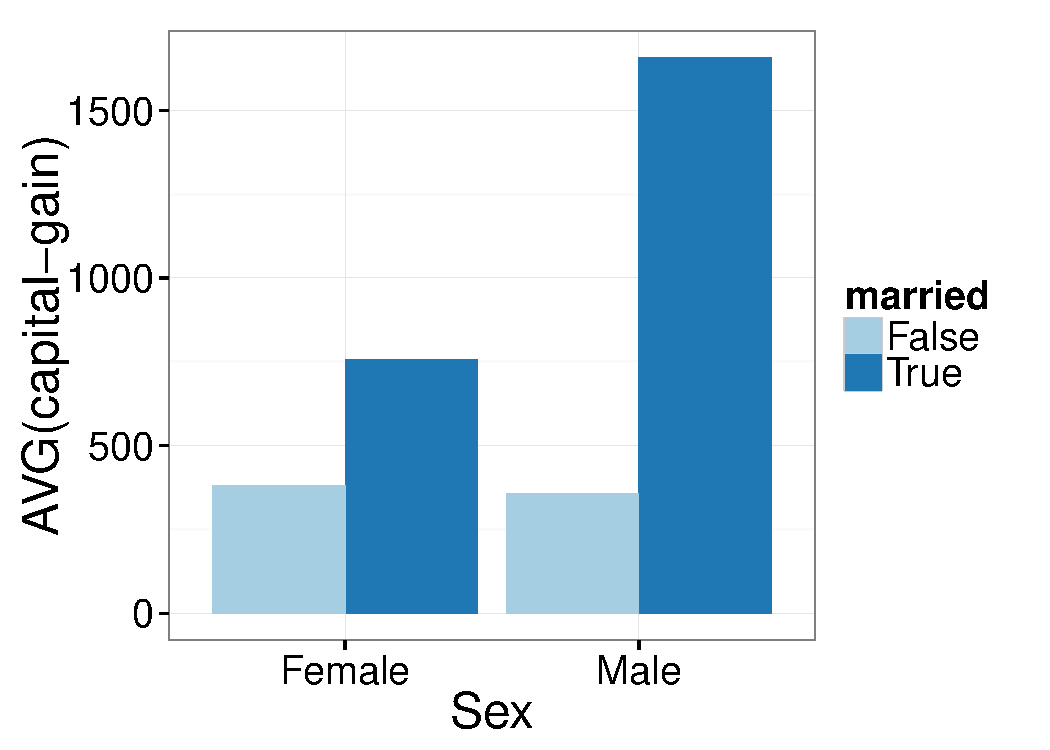
\includegraphics[width=4cm] {Images/HUHI_sex_avg_cap_gain.pdf}}
		\caption{Interesting Visualization}
		\label{fig:interesting_viz} 
	\end{subfigure}
	\begin{subfigure}{0.49\linewidth}
		\centering
		{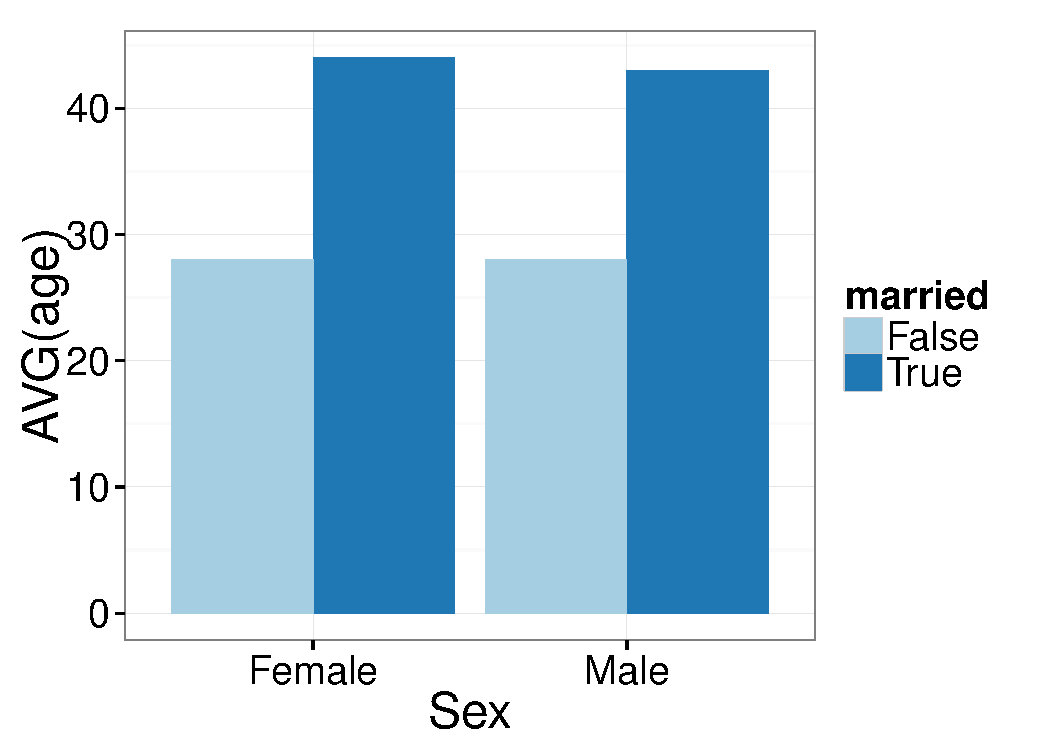
\includegraphics[width=4cm] {Images/LULI_sex_avg_age.pdf}}
		\caption{Uninteresting Visualization}
		\label{fig:uninteresting_viz}
	\end{subfigure}
	\vspace{-10pt}
	\caption{Motivating Example}
	\label{fig:intro}
	\vspace{-10pt}
\end{figure}

%What might make one of these visualizations ``interesting'' or valuable for the 
%task at hand depends on a number of factors.
\resolved{
\srm{I suggested below that our user studies show that users like our metric. Do we believe this?}
\agp{rewrote to remove preference}	
}
% Of the entire set of possible visualizations, only a small fraction of visualizations
% show trends and information relevant for the specific task.
We have identified that across many analyses, 
visualizations that show trends in the target 
data (i.e., {\em unmarried} adults) that 
deviate from trends in reference data (i.e., {\em married}
adults) are potentially interesting to analysts.
For example, 
from our user study (Section \ref{sec:user_study}), 
we know that for this particular task involving the Census dataset,
analysts find the visualization in Figure \ref{fig:interesting_viz} 
interesting since it depicts an aspect of the data for unmarried adults 
that is significantly different from the equivalent aspect
for married adults.
Specifically, the chart show that although capital gain 
for female and male unmarried adults 
is approximately equal, capital gain for female, 
married adults is only half that of male, 
married adults.
%Since this observation is relevant to the analytical task and merits further investigation,
%analysts find the visualization interesting.
The same user study also shows that Figure \ref{fig:uninteresting_viz} 
is a visualization that 
analysts do not find interesting. 
Note that this chart shows that age does {\em not} show different trends between unmarried
and married adults.
% In the case of app analytics, this underlying distribution might be metrics for
% all apps, versus the distribution of particular metrics specifically in BadApp.
% As an example, our user studies suggest that users will find the visualization of load times by carrier (Figure
% \ref{fig:staplerX}) more interesting if the trend for load times across all
% apps shows the {\it opposite} trend (e.g. Figure \ref{fig:staplerX-a}), and less interesting if the overall trend for all apps followed a similar trend.
% (Figure \ref{fig:staplerX-b}).  
\end{example}

%Since our goal with \SeeDB is to make visual analytics faster, we adopt a metric
%that prefers visualizations that show interesting or surprising trends in data.
%Specifically, we are motivated by the following observation:
%\begin{quotation}
%The greatest value of a picture is when it forces us to notice what we never expected to see.
%\end{quotation} 
%\begin{flushright} 
%- John Tukey, Exploratory Data Analysis 1977
%\end{flushright}

% While this utility metric is an example of a simple recommendation metric,
% it plays an important role in recommendations when 
% there is no prior history --- and therefore no user preferences
% or understanding of context.
% This special case is especially appropriate when the analyst
% is not very familiar with a dataset and is analyzing it for the first time.
% That said, in Section~\ref{sec:discussion}, we describe how our deviation-based
% metric can, in fact, encompass a large number of data-driven utility metrics and
% can be seamlessly extended to support other dimensions such as user preferences.

%These include other functions based on data distribution (e.g. scoring based on 
%statistical summaries) and functions that measure utility along {\em 
%dimensions} other than data distribution. 
%These utility dimensions 
%include aesthetics (e.g. is a bar plot more appropriate than a 
%scatter plot), context (e.g. prior knowledge that only female patients visit the
%obstetrics department), and user preference (e.g. in the sales dataset, profit is
%the most relevant attribute).
%Exploration of each of these dimensions forms a distinct body of work.

% functions 
% that can be used to score the utility of a 
% visualization; these can be different functions based on data distribution (e.g. scoring
% based on statistical summaries of data or outlier detection) or functions that take
% orthogonal {\em dimensions} of utility into account, e.g., user preferences, aesthetics, and context.
% The pruning framework we propose in Section \ref{sec:in_memory_execution_engine} can be applied to a large set of 
% functions derived from data distribution, and \SeeDB
% can support these metrics without any changes. \mpv{Verify true? Add characterization
% of metrics}
% Investigations of the other dimensions of utility form a distinct body of work, and
% we leave these explorations for future work.
% \mpv{keep? In section \ref{sec:discission}, we outline some means by which \SeeDB may be 
% extended to support these metrics.}
% We leave the investigation of other dimensions of utility to future work, but outline
% in Section \ref{sec:discussion} some means by which \SeeDB may be extended to support them.

% Due to the scale of data, most common visualizations show aggregate summaries of data
% as opposed to individual records (e.g. average sales by state vs. sales of each store 
% in every state).
% Consequently, our current implementation of \SeeDB\ recommends visualizations that show aggregate 
% summaries of data.

% Of course, there are a variety of other possible data-driven metrics for quality or utility
% of a visualization.
% For instance, one might focus on visualizations that show order statistics or anomalies~\cite{DBLP:conf/avi/KandelPPHH12}. 
% These would be important for spotting, for example, unusual spikes in machine load.
% Similarly, drawing upon the literature on data cubes, one might choose visualizations that highlight aggregates that
% are unusual given the remaining values in the cube~\cite{DBLP:conf/vldb/Sarawagi00}.
% Finally, one might choose to not aggregate any values but show correlations between attributes by plotting a random
% sampling of data-points.  Incorporating these other types of visualizations into our framework is an interesting
% direction for future work.



% The majority of visualizations that are generated in visualization systems are based on aggregate summaries of the
% underlying data.
% As a result, the {\it trends} we study are the results of grouping and aggregation applied to a given dataset.


% Thus, the recommendation algorithm used by \SeeDB\ works as follows: given a dataset $D$ and a query $Q$
% indicating the subset of data of interest to the analyst, \SeeDB finds the visualizations of $Q$ that 
% show the highest deviation between trends in $Q$ and trends in $D$. 
% Specifically, \SeeDB considers visualizations that can be constructed via a combinations of grouping and 
% aggregation applied to $Q$.
The example above suggests that visualizations that depict
deviations from a reference visualization are potentially interesting to analysts;
our goal in the current paper is to build a system 
that uses deviation as a means to identify
the most interesting visualizations from a large set of potential visualizations.
No existing system that we are aware of makes use of variation from a reference dataset
to recommend visualizations.  
Current visualization packages like Spotfire~\cite{Ahlberg:1996:SIE:245882.245893} and Tableau~\cite{tableau,polaris} have limited capabilities for 
recommending visualizations.
Their recommendations only implement rules-of-thumb 
regarding chart aesthetics such as choice of
chart type, colors and marks, drawing from
classical work by Mackinlay~\cite{Mackinlay:1986:ADG:22949.22950} and Cleveland and Gill~\cite{cleveland1984graphical}.
As noted previously, in addition to our deviation-based metric,
there are of course many other dimensions (aesthetics, user
preferences, etc.) that can influence the perceived utility of a
visualization, a few of which we discuss in Section
\ref{sec:discussion}, leaving a detailed investigation of such metrics
for future work.
%No existing system that we are aware of leverages insights about the underlying data
%into make visualization recommendations. \mpv{does this sound ok?} \agp{I would start with
%the statement that no current system supports the recommending of interesting visualizations
%where the target dataset shows some discrepancies not found in the underlying data.
%Then say the first two lines.}

% In this paper, we present \SeeDB, an end-to-end visualization platform 
% where analysts can both generate their own visualizations (like Tableau or Spotfire), 
% or get data-driven recommendations on demand.
Our implementation of \SeeDB incorporates an end-to-end data querying na 
visualization environment that allows where analysts to manually generate 
their own visualizations (like Tableau or Spotfire), or get data-driven recommendations on demand, which
can be further refined using the manual interface.
We chose to support both automated and manual interaction in \SeeDB because we 
believe that a {\em mixed-initiative interface}~\cite{mixed_initiative} is essential for keeping 
analysts in the loop and allowing them to drive the analysis process.
\SeeDB, is built as a middleware layer that can run on any 
relational database system.
In this paper, we develop and validate the use of  
two orthogonal techniques to make the problem
of recommending visualizations tractable:
\begin{denselist}
\item {\em Sharing Computation.} 
We develop a suite of multi-query optimization techniques to share computation
among the candidate visualizations,
reducing time taken by 20X.
\item {\em Pruning Computation.}
We develop pruning techniques to avoid wasting computation
on obviously low-utility visualizations, adapting
techniques from traditional 
  confidence-interval-based~\cite{hoeffding1963probability} 
  top-$k$ ranking and
  multi-armed bandits~\cite{bandits},
  further reducing time taken by 5X.
\end{denselist}
Lastly, we develop a general {\em phase-based execution framework}
that allows us to leverage the benefits of these two techniques
in tandem, reducing the time for execution by over 100X and
making many recommendations feasible in real-time.
We conclude by presenting an experimental evaluation of \SeeDB 
via both a performance study and a user study.
In summary, the contributions of this paper are:

% efficiently manages the search
% for data-driven visualization recommendations at interactive time scales.
% We show that \SeeDB can be implemented on top of a traditional relational database,
% allowing it to take advantage of the benefits of the interfaces and features
% relation engines expose.
% Doing this, however,
% also leads to inefficiencies that arise due to the requirement that data be
% accessed via SQL.   
% We manage these inefficiencies by introducing two classes of optimizations:
% {\em sharing-based} optimizations, that try to batch
% and share as much computation as possible to minimize the number of SQL queries,
% and {\em pruning-based optimizations}, that try to avoid
% as much unnecessary work as possible, and discarding candidate aggregate views
% that are of low utility.
\begin{denselist}
%  \item We design \SeeDB as a system for data-driven visualization recommendations.
%  We explore and evaluate two distinct implementations of the system, one as a
%  wrapper around a database and another a custom solution (Section~\ref{sec:system_architecture}).
  \item We build a system that uses deviation from reference as a criterion for finding the
  top-$k$ most interesting visualizations for an analytical task (Section~\ref{sec:problem_statement}).

  \item We present the design of \SeeDB as a middleware layer that can run on any SQL-compliant DBMS 
  (Section~\ref{sec:system_architecture}).
  
  \item We describe \SeeDB's optimizer (Section~\ref{sec:optimizer}), that uses
  sharing techniques to share computation 
  across visualizations (Section~\ref{sec:sharing_opt}) and
  pruning techniques to avoid computation of low-utility visualizations
  (Section~\ref{sec:pruning_opt}).
  

  \item We evaluate the performance of \SeeDB and demonstrate that \SeeDB
  can identify high-utility visualizations with high accuracy and at interactive time scales
  (Section~\ref{sec:experiments}).

  \item We present the results of a controlled user study that validates our deviation-based 
  utility metric, and evaluates \SeeDB against a manual chart construction tool 
  showing that \SeeDB can speed up identification of interesting 
  visualizations (Section \ref{sec:user_study}).

  \item We describe how we can extend \SeeDB to capture other utility criteria
  beyond deviation (Section~\ref{sec:discussion}).
\end{denselist}

\noindent Finally, we note that the vision for \SeeDB\ was described 
in a vision paper~\cite{DBLP:conf/vldb/Parameswaran2013} and presented 
as a demonstration~\cite{DBLP:journals/pvldb/VartakMPP14}, 
but neither of these short papers described detailed, concrete algorithms or
architectures, or 
presented any form of evaluation.
Specifically, the present work builds 
upon the \SeeDB vision by proposing a novel, general-purpose phase-based
execution framework that can leverage both 
sharing and pruning optimizations (that were described very briefly
in the short papers)
and presenting both a performance study of the system as well as a extensive
user study demonstrating the efficacy of our system in aiding analysis.


